

\tikzset{every picture/.style={line width=0.75pt}} %set default line width to 0.75pt        

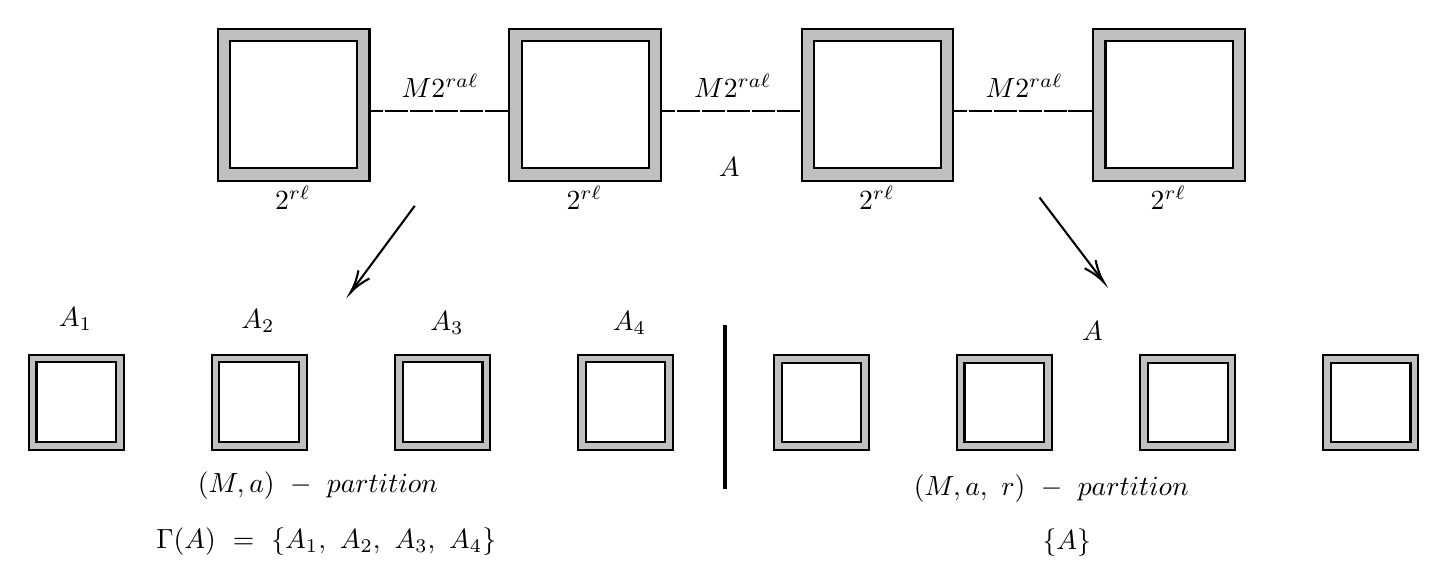
\begin{tikzpicture}[x=0.75pt,y=0.75pt,yscale=-1,xscale=1]
%uncomment if require: \path (0,289); %set diagram left start at 0, and has height of 289

%Shape: Rectangle [id:dp5324416495294659] 
\draw  [fill={rgb, 255:red, 155; green, 155; blue, 155 }  ,fill opacity=0.63 ] (386.36,19.67) -- (459.53,19.67) -- (459.53,92.84) -- (386.36,92.84) -- cycle ;
%Shape: Rectangle [id:dp5500278606044966] 
\draw  [fill={rgb, 255:red, 255; green, 255; blue, 255 }  ,fill opacity=1 ] (392.34,25.65) -- (453.55,25.65) -- (453.55,86.86) -- (392.34,86.86) -- cycle ;
%Shape: Rectangle [id:dp2596179707695043] 
\draw  [dash pattern={on 4.5pt off 4.5pt}] (319.59,59.27) -- (386.01,59.27) -- (386.01,59.22) -- (319.59,59.22) -- cycle ;
%Shape: Rectangle [id:dp24913467772666475] 
\draw  [fill={rgb, 255:red, 155; green, 155; blue, 155 }  ,fill opacity=0.63 ] (526.82,19.67) -- (600,19.67) -- (600,92.84) -- (526.82,92.84) -- cycle ;
%Shape: Rectangle [id:dp0593609628931453] 
\draw  [fill={rgb, 255:red, 255; green, 255; blue, 255 }  ,fill opacity=1 ] (532.8,25.65) -- (594.02,25.65) -- (594.02,86.86) -- (532.8,86.86) -- cycle ;
%Shape: Rectangle [id:dp6930367358141787] 
\draw  [dash pattern={on 4.5pt off 4.5pt}] (460.05,59.27) -- (526.48,59.27) -- (526.48,59.22) -- (460.05,59.22) -- cycle ;
%Shape: Rectangle [id:dp3891355185035541] 
\draw  [fill={rgb, 255:red, 155; green, 155; blue, 155 }  ,fill opacity=0.63 ] (105,19.67) -- (178.18,19.67) -- (178.18,92.84) -- (105,92.84) -- cycle ;
%Shape: Rectangle [id:dp18348616469112367] 
\draw  [fill={rgb, 255:red, 255; green, 255; blue, 255 }  ,fill opacity=1 ] (110.98,25.65) -- (172.2,25.65) -- (172.2,86.86) -- (110.98,86.86) -- cycle ;
%Shape: Rectangle [id:dp8439231420612681] 
\draw  [fill={rgb, 255:red, 155; green, 155; blue, 155 }  ,fill opacity=0.63 ] (245.47,19.67) -- (318.64,19.67) -- (318.64,92.84) -- (245.47,92.84) -- cycle ;
%Shape: Rectangle [id:dp8890085997124306] 
\draw  [fill={rgb, 255:red, 255; green, 255; blue, 255 }  ,fill opacity=1 ] (251.45,25.65) -- (312.66,25.65) -- (312.66,86.86) -- (251.45,86.86) -- cycle ;
%Shape: Rectangle [id:dp10785414278689243] 
\draw  [dash pattern={on 4.5pt off 4.5pt}] (178.7,59.27) -- (245.13,59.27) -- (245.13,59.22) -- (178.7,59.22) -- cycle ;
%Shape: Rectangle [id:dp14308030153782791] 
\draw  [fill={rgb, 255:red, 155; green, 155; blue, 155 }  ,fill opacity=0.63 ] (190.49,176.67) -- (236.39,176.67) -- (236.39,222.57) -- (190.49,222.57) -- cycle ;
%Shape: Rectangle [id:dp9137494636300982] 
\draw  [fill={rgb, 255:red, 255; green, 255; blue, 255 }  ,fill opacity=1 ] (194.24,180.42) -- (232.64,180.42) -- (232.64,218.82) -- (194.24,218.82) -- cycle ;
%Shape: Rectangle [id:dp15646249724623273] 
\draw  [fill={rgb, 255:red, 155; green, 155; blue, 155 }  ,fill opacity=0.63 ] (278.6,176.67) -- (324.5,176.67) -- (324.5,222.57) -- (278.6,222.57) -- cycle ;
%Shape: Rectangle [id:dp577612871496954] 
\draw  [fill={rgb, 255:red, 255; green, 255; blue, 255 }  ,fill opacity=1 ] (282.35,180.42) -- (320.75,180.42) -- (320.75,218.82) -- (282.35,218.82) -- cycle ;
%Shape: Rectangle [id:dp8898021024931992] 
\draw  [fill={rgb, 255:red, 155; green, 155; blue, 155 }  ,fill opacity=0.63 ] (14,176.67) -- (59.9,176.67) -- (59.9,222.57) -- (14,222.57) -- cycle ;
%Shape: Rectangle [id:dp9806302049467206] 
\draw  [fill={rgb, 255:red, 255; green, 255; blue, 255 }  ,fill opacity=1 ] (17.75,180.42) -- (56.15,180.42) -- (56.15,218.82) -- (17.75,218.82) -- cycle ;
%Shape: Rectangle [id:dp458396485821043] 
\draw  [fill={rgb, 255:red, 155; green, 155; blue, 155 }  ,fill opacity=0.63 ] (102.11,176.67) -- (148.01,176.67) -- (148.01,222.57) -- (102.11,222.57) -- cycle ;
%Shape: Rectangle [id:dp23889693035006787] 
\draw  [fill={rgb, 255:red, 255; green, 255; blue, 255 }  ,fill opacity=1 ] (105.86,180.42) -- (144.26,180.42) -- (144.26,218.82) -- (105.86,218.82) -- cycle ;
%Shape: Rectangle [id:dp5244573854005878] 
\draw  [fill={rgb, 255:red, 155; green, 155; blue, 155 }  ,fill opacity=0.63 ] (549.49,176.77) -- (595.39,176.77) -- (595.39,222.67) -- (549.49,222.67) -- cycle ;
%Shape: Rectangle [id:dp33659917623157787] 
\draw  [fill={rgb, 255:red, 255; green, 255; blue, 255 }  ,fill opacity=1 ] (553.24,180.52) -- (591.64,180.52) -- (591.64,218.92) -- (553.24,218.92) -- cycle ;
%Shape: Rectangle [id:dp4477759165612456] 
\draw  [fill={rgb, 255:red, 155; green, 155; blue, 155 }  ,fill opacity=0.63 ] (637.6,176.77) -- (683.5,176.77) -- (683.5,222.67) -- (637.6,222.67) -- cycle ;
%Shape: Rectangle [id:dp008960265086033203] 
\draw  [fill={rgb, 255:red, 255; green, 255; blue, 255 }  ,fill opacity=1 ] (641.35,180.52) -- (679.75,180.52) -- (679.75,218.92) -- (641.35,218.92) -- cycle ;
%Shape: Rectangle [id:dp5482577070086769] 
\draw  [fill={rgb, 255:red, 155; green, 155; blue, 155 }  ,fill opacity=0.63 ] (373,176.77) -- (418.9,176.77) -- (418.9,222.67) -- (373,222.67) -- cycle ;
%Shape: Rectangle [id:dp620593794066499] 
\draw  [fill={rgb, 255:red, 255; green, 255; blue, 255 }  ,fill opacity=1 ] (376.75,180.52) -- (415.15,180.52) -- (415.15,218.92) -- (376.75,218.92) -- cycle ;
%Shape: Rectangle [id:dp1271602148339841] 
\draw  [fill={rgb, 255:red, 155; green, 155; blue, 155 }  ,fill opacity=0.63 ] (461.11,176.77) -- (507.01,176.77) -- (507.01,222.67) -- (461.11,222.67) -- cycle ;
%Shape: Rectangle [id:dp512454895948047] 
\draw  [fill={rgb, 255:red, 255; green, 255; blue, 255 }  ,fill opacity=1 ] (464.86,180.52) -- (503.26,180.52) -- (503.26,218.92) -- (464.86,218.92) -- cycle ;
%Shape: Rectangle [id:dp5220547084154457] 
\draw   (349,162.84) -- (350,162.84) -- (350,241) -- (349,241) -- cycle ;
%Straight Lines [id:da3745574378116445] 
\draw    (200,105) -- (170.19,145.24) ;
\draw [shift={(169,146.84)}, rotate = 306.53] [color={rgb, 255:red, 0; green, 0; blue, 0 }  ][line width=0.75]    (10.93,-3.29) .. controls (6.95,-1.4) and (3.31,-0.3) .. (0,0) .. controls (3.31,0.3) and (6.95,1.4) .. (10.93,3.29)   ;
%Straight Lines [id:da48070403104101245] 
\draw    (501,101) -- (530.79,140.25) ;
\draw [shift={(532,141.84)}, rotate = 232.8] [color={rgb, 255:red, 0; green, 0; blue, 0 }  ][line width=0.75]    (10.93,-3.29) .. controls (6.95,-1.4) and (3.31,-0.3) .. (0,0) .. controls (3.31,0.3) and (6.95,1.4) .. (10.93,3.29)   ;

% Text Node
\draw (333.04,40.2) node [anchor=north west][inner sep=0.75pt]    {$M2^{ra\ell }$};
% Text Node
\draw (412.57,94.1) node [anchor=north west][inner sep=0.75pt]    {$2^{r\ell }$};
% Text Node
\draw (473.5,40.2) node [anchor=north west][inner sep=0.75pt]    {$M2^{ra\ell }$};
% Text Node
\draw (553.03,94.1) node [anchor=north west][inner sep=0.75pt]    {$2^{r\ell }$};
% Text Node
\draw (131.21,94.1) node [anchor=north west][inner sep=0.75pt]    {$2^{r\ell }$};
% Text Node
\draw (192.15,40.2) node [anchor=north west][inner sep=0.75pt]    {$M2^{ra\ell }$};
% Text Node
\draw (271.68,94.1) node [anchor=north west][inner sep=0.75pt]    {$2^{r\ell }$};
% Text Node
\draw (94,231.4) node [anchor=north west][inner sep=0.75pt]    {$( M,a) \ -\ \text{partition}$};
% Text Node
\draw (74,258.4) node [anchor=north west][inner sep=0.75pt]    {$\Gamma ( A) \ =\ \{A_{1} ,\ A_{2} ,\ A_{3} ,\ A_{4}\}$};
% Text Node
\draw (439,233.06) node [anchor=north west][inner sep=0.75pt]    {$( M,a,\ r) \ -\ \text{partition}$};
% Text Node
\draw (501,259.06) node [anchor=north west][inner sep=0.75pt]    {$\{A\}$};
% Text Node
\draw (27,152.4) node [anchor=north west][inner sep=0.75pt]    {$A_{1}$};
% Text Node
\draw (115,153.4) node [anchor=north west][inner sep=0.75pt]    {$A_{2}$};
% Text Node
\draw (206,154.4) node [anchor=north west][inner sep=0.75pt]    {$A_{3}$};
% Text Node
\draw (294,154.4) node [anchor=north west][inner sep=0.75pt]    {$A_{4}$};
% Text Node
\draw (345,80.4) node [anchor=north west][inner sep=0.75pt]    {$A$};
% Text Node
\draw (520,159.4) node [anchor=north west][inner sep=0.75pt]    {$A$};


\end{tikzpicture}